
\section{Trójkąty}
\subsection{Trójkąty}

\subsubsection{Cechy przystawania}
Cechy przystawania
\loremipsum
Hartshorne s. 99

%

,,\emph{Pons asinorum}'', czyli most osłów, to tradycyjna nazwa twierdzenia (I.5), że kąty przy podstawie trójkąta równoramiennego są równe.
Ci, którzy nie są w stanie samodzielnie przeprowadzić jego dedukcyjnego dowodu opartego na własnościach trójkątów przystających, nie mogą przekroczyć mostu i studiować dalej geometrii.
Bardziej przyziemnie Coxeter \cite[s. 22-24]{coxeter_1967} zauważa, że rysunek wykonany przez Euklidesa przypomni most.
Wśród konsekwencji wymienia wyniki z~Elementów: (III.3), (III.20), (III.21), (III.22), (III.32), (VI.2), (VI.4), a potem (III.35), (III.36), (VI.19), co prowadzi do dowodu twierdzenia Pitagorasa, czyli (I.47). % TODO: sprawdzić, czy numeracja moja i Coxetera jest taka sama.
\index{twierdzenie!Pitagorasa}%

\begin{figure}[H] \centering
\begin{comment}
\begin{tikzpicture}[scale=.5]
    \tkzDefPoint(90:-1){A}
    \tkzDefPoint(-55:5){C}
    \tkzDefPoint(235:5){B}
    \tkzDefPoint(-90:8){X}

    \tkzLabelPoint[above](A){$A$}
    \tkzLabelPoint[left](B){$B$}
    \tkzLabelPoint[right](C){$C$}
    \tkzInterLC(A,B)(A,X) \tkzGetPoints{XX}{D} % line and circle
    \tkzLabelPoint[left](D){$D$}
    \tkzDefLine[parallel=through D](B,C) \tkzGetPoint{XXX}
    \tkzInterLL(D,XXX)(A,C) \tkzGetPoint{E} % line and circle
    \tkzLabelPoint[right](E){$E$}
    
    \tkzMarkSegments[mark=|](A,B A,C)
    \tkzMarkSegments[mark=||](B,D C,E)
    \tkzDrawLines[add= 0 and 0, line width=0.2mm](B,E C,D)
    \tkzDrawLines[add= 0 and 0.5, line width=0.2mm](B,D C,E)
    \tkzDrawPolygon[line width=0.5mm](A,B,C)
    \tkzDrawPoints[size=4,color=black,fill=black!50](A,B,C,D,E)
\end{tikzpicture}
\end{comment}
    \caption{most osłów}
\end{figure}

Pierwsze dowody tego faktu podadzą jeszcze Euklides, komentujący jego prace Proklos, a także (dużo krócej\footnote{Pappus zauważa, że trójkąt $\triangle ABC$ przystaje do siebie $\triangle ACB$, więc stosowne kąty przy podstawie też są przystajace.}) Pappus z Aleksandrii.
\index[persons]{Proklos zwany Diadochem}%
\index[persons]{Pappus z Aleksandrii}%
Przyszłość przyniesie jeszcze jedno uzasadnienie, zaczynające się od wykreślenia dwusiecznej z kąta przy wierzchołku.
\index{dwusieczna}%
Euklides nie zrobi tego przede wszystkim ze względu na kolejność wykładanego materiału: dwusieczna pojawi się cztery tezy później, a nie można korzystać z wyników, których prawdziwości dopiero się pokaże.

O pons asinorum nie wspomina żaden szkolny podręcznik geometrii \texttt{:(}
Pojawia się u Bogdańskiej, Neugebauera \cite[s. 9]{neugebauer_2018}.

% PRZECZYTANO: https://en.wikipedia.org/wiki/Pons_asinorum

%

%

Zajmiemy się teraz (I.20).

\begin{proposition}[nierówność trójkąta]
\index{nierówność!trójkąta}%
	Niech $ABC$ będzie trojkątem.
	Wtedy suma odcinków $AB$ i $BC$ jest dłuższa niż $AC$.
\end{proposition}
% PRZECZYTANO: https://en.wikipedia.org/wiki/Triangle_inequality

\begin{proof}
	Wynika to ze wzoru Herona (fakt \ref{prp_heron}) i tego, że pole trójkąta jest nieujemne.
\end{proof}

\begin{corollary}
	Niech $a \ge b \ge c$ będą bokami trójkąta.
	Wtedy
	% \begin{equation}
	% 	1 < \frac{a + c}{b} < 3 
	% \end{equation}
	% oraz
	\begin{equation}
		1 \le \min \left(\frac ab, \frac bc\right) \le \phi = \frac {1 + \sqrt 5}{2}.
		% American Mathematical Monthly, pp. 49-50, 1954. 
	\end{equation}
\end{corollary}

Nierówność trójkąta nie jest wnioskiem z aksjomatów I1-I3, B1-B4, C1-C3, ponieważ nie zachodzi w następującym modelu (ukradniętym Hartshorne'owi \cite[s. 90]{hartshorne2000}):

\begin{example}
	Rozpatrujemy zbiór $\mathbb R^2$ jako płaszczyznę ze standardowymi punktami oraz prostymi, ale niestandardową metryką
	\begin{equation}
		d((x_1, y_1), (x_2, y_2)) = \begin{cases}
			\sqrt{(x_1-x_2)^2 + (y_1-y_2)^2} & \text{jeśli } x_1 = x_2 \vee y_1 = y_2, \\
			2 \sqrt{(x_1-x_2)^2 + (y_1-y_2)^2} & \text{w przeciwnym wypadku}
		\end{cases}.
	\end{equation}
	Wtedy nierówność trójkąta nie zachodzi.
\end{example}

% section{Problemy Fagnano i Fermata}
% https://en.wikipedia.org/wiki/Fagnano's_problem

\begin{problem}[zadanie Fagnano]
	Dany jest trójkąt ostrokątny $ABC$.
	Wpisać w niego trójkąt $UVW$ o możliwie najmniejszym obwodzie.
\index{zadanie!Fermata}%
\end{problem}

Coxeter \cite[s. 36, 37]{coxeter_1967} pokaże tak jak Fejer, że rozwiązaniem zadania jest trójkąt spodkowy (zwany ortycznym).
Audin \cite[s. 101]{audin_2003} podaje ten fakt w formie ćwiczenia. % todo: fagnano czy gemrat?

\begin{problem}[zadanie Fermata]
	\label{punkt_fermata}
	Dany jest trójkąt ostrokątny $ABC$.
	Znaleźć punkt $F$ taki, by suma $|FA| + |FB| + |FC|$ była możliwie najmniejsza.
\index{zadanie!Fermata}%
\end{problem}

\todofoot{Zadanie Fermata -- Neugebauer, s. 117.}

Powyższe zadanie rozwiąże Evangelista Torricelli (dlatego też punkt $F$ nazywa się czasem punktem Torricellego; robi tak Guzicki \cite[s. 224-228]{guzicki_2021}), który dostanie je w formie wyzwania od Fermata.
\index[persons]{Torricelli, Evangelista}%.
Rozwiązanie opublikuje student Torricelliego, Vincenzo Viviani, w 1659 roku.
\index[persons]{Viviani, Vincenzo}
% TODO: Johnson, R. A. Modern Geometry: An Elementary Treatise on the Geometry of the Triangle and the Circle. Boston, MA: Houghton Mifflin, pp. 221-222, 1929.
Coxeter \cite[s. 37]{coxeter_1967} przytoczy rozwiązanie Hofmanna\todofoot{J E Hoffman, Elementare Losung einer Mimimumsaufgabe 1929}
\index{zadanie!Fagnano}

%

%

Najważniejszym twierdzeniem dotyczącym trójkątów prostokątnych jest twierdzenie Pitagorasa oraz twierdzenie do niego odwrotne.
Piszą o~nim Guzicki \cite[s. 160]{guzicki_2021}.

% PRZECZYTANO: https://en.wikipedia.org/wiki/Pythagorean_theorem

\begin{theorem}[Pitagorasa]
\label{theorem_pythagorean}%
    Niech $ABC$ będzie trójkątem prostokątnym, w~którym kąt przy wierzchołku $C$ jest prosty.
    \begin{center}
\begin{comment}
        \begin{tikzpicture}[scale=.4]
        %\tkzInit[xmin=-0.5,xmax=6.5, ymin=-0.5,ymax=4.5]
        % \tkzClip
        \tkzDefPoint(105:3){A}
        \tkzDefPoint(285:3){B}
        \tkzDefPoint(35:3){C}
        \tkzDefPoint(35:4.75){CC}
        \tkzMarkRightAngle[size=0.5](A,C,B)

        \tkzLabelPoint[above left](A){$A$}
        \tkzLabelPoint[below](B){$B$}
        \tkzLabelPoint[below left](CC){$C$}
        \tkzDefSquare(B,A)
        \tkzDrawPolygon[fill=black!50](B,A,tkzFirstPointResult, tkzSecondPointResult)
        \tkzDefSquare(C,B)
        \tkzDrawPolygon[fill=black!25](C,B,tkzFirstPointResult, tkzSecondPointResult)
        \tkzDefSquare(A,C)
        \tkzDrawPolygon[fill=black!25](A,C,tkzFirstPointResult, tkzSecondPointResult)
        \tkzDrawPolygon[line width=0.4mm](A,B,C)
    \end{tikzpicture}
\end{comment}
    \end{center}
    Wtedy suma pól jasnych kwadratów jest równa polu ciemnego kwadratu:
    \begin{equation}
        |AC|^2 + |BC|^2 = |AB|^2.
    \end{equation}
    Odwrotnie, jeśli $ABC$ jest trójkątem takim, że $|AC|^2 + |BC|^2 = |AB|^2$, to trójkąt ten jest prostokątny, zaś kąt przy wierzchołku $C$ jest prosty.
\end{theorem}

Powyższe twierdzenie przypiszemy kiedyś Pitagorasowi z~Samos, choć nie wiemy dokładnie, kto i~kiedy odkryje je jako pierwszy.
\index[persons]{Pitagoras z Samos}%
Będzie powszechnie stosowane w~okresie Starego Babilonu (XX-XVI wiek p.n.e.), a~więc na długo przed narodzinami Pitagorasa; pojawi się też w~indyjskich i~chińskich tekstach matematycznych.
Papirus Berlin 6619 spisany ok. 1800 roku p.n.e. na terenach państwa egipskiego zawrze zadanie, którego rozwiązaniem jest trójka $(6, 8, 10)$.
\index{papirus Berlin 6619}%
Jest jeszcze babilońska tabliczka Plimpton 322, także spisana ok. 1800 roku p.n.e., gdzie pojawia się trójka
\begin{equation}
    12709^2 + 13500^2 = 18541^2,
\end{equation}
co sugeruje, że jej autor znał pewną systematyczną metodę.
\index{tabliczka Plimpton 322}%

Być może twierdzenie Pitagorasa ma więcej znanych dowodów niż jakiekolwiek inne (poza prawem wzajemności reszt kwadratowych).
Będzie ich tak bardzo bez liku, że nie wiadomo, ile dokładnie.
Niektóre opierają się na rozcięciu pewnej układanki na fragmenty, przestawieniu ich i~zbudowaniu innego kształtu.
Inne korzystają z podobieństwa trójkątów.
Dowód Euklidesa urzekł nas tak bardzo swoją pomysłowością, że będzie jedynym, jaki przedstawimy w~całej książce!
\index{zasada!Cavalieriego}

\begin{proof}
    Niech $\triangle ABC$ będzie trójkątem prostokątnym, z kątem prostym przy wierzchołku $C$.
    Na bokach $BC$, $AB$, $CA$ kreślimy kolejno kwadraty $BCDE$, $ABFG$, $ACHI$ (konstrukcja kwadratu Euklidesa korzysta z postulatu równoległości).

    \begin{center}
\begin{comment}
            \begin{tikzpicture}[scale=.4]
        %\tkzInit[xmin=-0.5,xmax=6.5, ymin=-0.5,ymax=4.5]
        % \tkzClip
        \tkzDefPoint(105:3){A}
        \tkzDefPoint(285:3){B}
        \tkzDefPoint(35:3){C}
        \tkzDefPoint(35:4.75){CC}

        \tkzLabelPoint[above left](A){$A$}
        \tkzLabelPoint[below](B){$B$}
        \tkzLabelPoint[below left](CC){$C$}
        \tkzDefSquare(B,A)
        \tkzGetPoints{G}{F}
        \tkzLabelPoint[below](F){$F$}
        \tkzLabelPoint[above](G){$G$}
        \tkzDefPointsBy[projection=onto A--B](C){K}
        \tkzDefPointsBy[projection=onto G--F](C){L}

        \tkzDrawPolygon[line width=0.3mm, fill=blue!10](A,K,L,G)
        \tkzDrawPolygon[line width=0.3mm, fill=red!10](B,K,L,F)
        \tkzDrawPolygon[line width=0.3mm](A,B,F,G)
        \tkzLabelPoint[below left](K){$K$}
        \tkzLabelPoint[left](L){$L$}


        \tkzDefSquare(C,B)
        \tkzGetPoints{E}{D}
        \tkzDrawPolygon[line width=0.3mm,fill=red!40](C,B,E,D)
        \tkzLabelPoint[above](D){$D$}
        \tkzLabelPoint[below](E){$E$}
        \tkzDefSquare(A,C)
        \tkzGetPoints{H}{I}
        \tkzDrawPolygon[line width=0.3mm, fill=blue!40](A,C,H,I)
        \tkzLabelPoint[above right](H){$H$}
        \tkzLabelPoint[above right](I){$I$}
        \tkzDrawSegments[line width=0.2mm](C,G)
        \tkzDrawSegments[line width=0.2mm, dashed](C,K)
        \tkzDrawSegments[line width=0.2mm](I,B)
        % \tkzMarkRightAngle[size=0.5](A,C,B)
        \tkzDrawPolygon[line width=0.5mm](A,B,C)
    \end{tikzpicture}
\end{comment}
    \end{center}
    Z punktu $C$ opuszczamy wysokość na przeciwprostokątną $AB$ i przedłużamy tak, by przecięła kwadrat $ABFG$ w punktach $K$ i $L$.
    Łączymy punkty $B$ i $I$ oraz $C$ i $G$.
    Otrzymane trójkąty $\triangle BAI$ oraz $\triangle GAC$ są przystające na mocy cechy bok-kąt-bok ($AB$, $\angle BAI$, $AI$ oraz $AG$, $\angle GAC$, $AC$).
    Niebieski prostokąt $AGLK$ (odpowiednio: kwadrat $ACHI$) ma dwukrotnie większe pole niż trójkąt $\triangle GAC$ (trójkąt $\triangle BAI$).
    (To jest zamaskowana zasada Cavalieriego!).
    \index{zasada Cavalieriego}%
    Zatem prostokąt $AGLK$ i~kwadrat $ACHI$ mają równe pola.
    
    Analogicznie pokazujemy, że czerwony prostokąt $BFLK$ i kwadrat $BCDE$ mają równe pola.
    Dodajemy dwie równości stronami i otrzymujemy, że suma pól kwadratów $ACIH$ oraz $BCDE$ jest równa polu kwadratu $ABFG$.
\end{proof}

Według legendy Hippazos z Metapontu odkryje, że przekątna kwadratu (albo, według innej legendy, pięciokąta) nie jest współmierna z~jego bokiem.
Niewymierność liczb $\sqrt{2}$ (albo $(1 + \sqrt 5) /2$) zrujnuje pogląd szkoły pitagorejskiej, że świat opiera się na liczbach (co dla ówczesnych znaczyć będzie: liczb naturalnych oraz ułamków z nich zbudowanych) i doprowadzi do utopienia Hippazosa.
\index[persons]{Hippazos z Metapontu}%
\index{utopienie}%
Ale jego śmierć nie cofnie rozłamu, jaki powstanie w szkole.

(Być może w tym miejscu warto dowiedzieć się o cegle Eulera.)

\begin{corollary}
    Długość przekątnej prostokąta o bokach długości $a$ i $b$ wynosi $\sqrt{a^2 + b^2}$.
\end{corollary}

Względnie pierwsze liczby naturalne $a, b, c$ takie, że $a^2 + b^2 = c^2$ nazywamy (pierwotną) trójką pitagorejską.
\index{trójka pitagorejska}%
Każdą taką trójkę można otrzymać biorąc względnie pierwsze liczby $m, n$ różnej parzystości takie, że $m > n$ i kładąc $a = m^2 - n^2$, $b = 2 mn$, $c = m^2 + n^2$.
Najmniejszą taką trójką jest $(3, 4, 5)$; inna legenda (nie było w niej ani smoków, ani Hippazosa) głosi, że Egipcjanie używali tego trójkąta do wyznaczania kątów prostych u podstawy piramid.

\begin{proposition}
    % TODO: rysunek z Guzickiego, stron 160
    Niech $\triangle ABC$ będzie trójkątem prostokątnym, z kątem prostym przy wierzchołku $C$:
        \begin{center}
\begin{comment}
    \begin{tikzpicture}[scale=.4]
        \tkzDefPoint(200:5){A}
        \tkzDefPoint(20:5){B}
        \tkzDefPoint(90:5){C}
        \tkzDefPointsBy[projection=onto A--B](C){D}
        \tkzLabelPoint[below left](200:5){A}
        \tkzLabelPoint[below right](22:5.3){B}
        \tkzLabelPoint[above](90:5.2){C}
        
        \tkzMarkRightAngle[size=0.8](A,C,B)
        \tkzDrawPolygons[line width=0.2mm](A,B,C)
        \tkzDrawSegment[dim={$\,\,p\,\,$,-8pt,transform shape,sloped}](A,D)
        \tkzDrawSegment[dim={$\,\,q\,\,$,-8pt,transform shape,sloped}](D,B)
        \tkzDrawSegment[dim={$\,\,b\,\,$,-8pt,transform shape,sloped}](C,A)
        \tkzDrawSegment[dim={$\,\,a\,\,$,-8pt,transform shape,sloped}](B,C)
        \tkzDrawPoints[size=3,color=black,fill=black!50](A,B,C)
        \tkzDrawSegment[dim={$\,\,h\,\,$,-0pt,transform shape,sloped}](C,D)
\end{tikzpicture}
\end{comment}
    \end{center}
    Mają wtedy miejsce następujące równości:
    \begin{equation}
        h = \frac{ab}{c}, \quad
        p = \frac{b^2}{c}, \quad
        q = \frac{a^2}{c}, \quad
        h^2 = pq.
    \end{equation}
\end{proposition}

Twierdzenie Pitagorasa znajduje zastosowanie także przy wyznaczaniu niektórych miejsc geometrycznych.

\begin{proposition}
    Dane są dwa różne punkty $A$ i $B$ na płaszczyźnie oraz liczba rzeczywista $c$ taka, że $2c > |AB|^2$.
    Miejscem geometrycznym punktów $P$ o własności $|AP|^2 + |BP|^2 = c$ jest okrąg o środku w środku odcinka $AB$ i promieniu $r = \frac 1 2 \sqrt{2c - |AB|^2}$.
\end{proposition}

\begin{proposition}
    Dane są dwa różne punkty $A$ i $B$ na płaszczyźnie oraz liczba rzeczywista $c$.
    Miejscem geometrycznym punktów $P$ o własności $|AP|^2 - |BP|^2 = c$ jest prosta prostopadła do prostej $AB$.
\end{proposition}

Patrz Guzicki \cite[s. 170-173]{guzicki_2021} (Guzicki wprowadza potem osie i środki potęgowe jak w~fakcie \ref{guzicki_6_11}, a następnie twierdzenie \ref{guzicki_6_13} (Carnota)).

Spirala Teodor(os)a z Cyreny składa się z trójkątów prostokątnych stykających się ze sobą wzdłuż boków.
\index{spirala Teodorusa}%
\index[persons]{Teodor(os) z Cyreny}%
Zaczynamy od trójkąta prostokątnego równoramiennego, o bokach długości $1$, $1$, $\sqrt{2}$, by następnie kreślić jednostkowy odcinek prostopadły do końca przeciwprostokątnej, łączymy go z~początkiem i powtarzamy (Teodoros zatrzyma się na trójkącie, którego najdłuższy bok to $\sqrt{17}$, ponieważ następny naszedłby na ten, od którego zaczynaliśmy).
\begin{center}
\begin{comment}
    \begin{tikzpicture}[scale=.7]
        \tkzDefPoints{0.0000000000000000/0.0000000000000000/sqrt0,1.0000000000000000/0.0000000000000000/sqrt1,1.0000000000000002/1.0000000000000000/sqrt2,0.2928932188134524/1.7071067811865475/sqrt3,-0.6927053408400360/1.8762087599123103/sqrt4,-1.6308097207961914/1.5298560894922923/sqrt5,-2.3149821631755443/0.8005358106787454/sqrt6,-2.6417995393402450/-0.1445516998920071/sqrt7,-2.5871641322679750/-1.1430580705747615/sqrt8,-2.1830320757712630/-2.0577587215594090/sqrt9,-1.4971125019181266/-2.7854360801498297/sqrt10,-0.6162802729096475/-3.2588646221072777/sqrt11,0.3663043810988235/-3.4446801158290160/sqrt12,1.3606978771718410/-3.3389371493126440/sqrt13,2.2867524231255560/-2.9615474595774080/sqrt14,3.0782592751547995/-2.3503871670266260/sqrt15,3.6851266321570497/-1.5555840398277552/sqrt16,4.0740226421139890/-0.634302381788492/sqrt17}
        \tkzDrawPolygons[line width=0.2mm](sqrt0,sqrt1,sqrt2 sqrt0,sqrt2,sqrt3 sqrt0,sqrt3,sqrt4 sqrt0,sqrt4,sqrt5 sqrt0,sqrt5,sqrt6 sqrt0,sqrt6,sqrt7 sqrt0,sqrt7,sqrt8 sqrt0,sqrt8,sqrt9 sqrt0,sqrt9,sqrt10 sqrt0,sqrt10,sqrt11 sqrt0,sqrt11,sqrt12 sqrt0,sqrt12,sqrt13 sqrt0,sqrt13,sqrt14 sqrt0,sqrt14,sqrt15 sqrt0,sqrt15,sqrt16 sqrt0,sqrt16,sqrt17)
        \tkzMarkRightAngle[size=0.25](sqrt0,sqrt1,sqrt2)
        \tkzMarkRightAngle[size=0.25](sqrt0,sqrt2,sqrt3)
        \tkzMarkRightAngle[size=0.25](sqrt0,sqrt3,sqrt4)
        \tkzMarkRightAngle[size=0.25](sqrt0,sqrt4,sqrt5)
        \tkzMarkRightAngle[size=0.25](sqrt0,sqrt5,sqrt6)
        \tkzMarkRightAngle[size=0.25](sqrt0,sqrt6,sqrt7)
        \tkzMarkRightAngle[size=0.25](sqrt0,sqrt7,sqrt8)
        \tkzMarkRightAngle[size=0.25](sqrt0,sqrt8,sqrt9)
        \tkzMarkRightAngle[size=0.25](sqrt0,sqrt9,sqrt10)
        \tkzMarkRightAngle[size=0.25](sqrt0,sqrt10,sqrt11)
        \tkzMarkRightAngle[size=0.25](sqrt0,sqrt11,sqrt12)
        \tkzMarkRightAngle[size=0.25](sqrt0,sqrt12,sqrt13)
        \tkzMarkRightAngle[size=0.25](sqrt0,sqrt13,sqrt14)
        \tkzMarkRightAngle[size=0.25](sqrt0,sqrt14,sqrt15)
        \tkzMarkRightAngle[size=0.25](sqrt0,sqrt15,sqrt16)
        \tkzMarkRightAngle[size=0.25](sqrt0,sqrt16,sqrt17)
\end{tikzpicture}
\end{comment}
\end{center}
Niektórzy nazywają otrzymaną figurę ślimakiem pitagorejskim.
\index{ślimak pitagorejski}

%
\subsubsection{Wzór Herona}

\index{wzór!Herona|(}
Guzicki \cite[s. 165-168]{guzicki_2021} wyprowadza wzór Herona z twierdzenia Pitagorasa.
\index{twierdzenie!Pitagorasa}
Oryginalny dowód Herona był dość skomplikowany, Guzicki \cite[s. 168-169]{guzicki_2021} wspomina o znacznie prostszym dowodzie geometrycznym, pochodzącym od Eulera.
\index[persons]{Euler, Leonhard}%
(Chociaż wynik przypisujemy obecnie Heronowi, został odkryty przez Archimedesa -- Coxeter \cite[s. 12]{coxeter_1991} odsyła do van der Waerdena \cite{MISSING_CITATION}).
% This remarkable expression, which we shall use in § 18.4, is attributed to Heron of Alexandria (about 60 a.d.), but it was really discovered by Archimedes. (See B. L. van der Waerden, Science Awakening, Oxford University Press, New York, 1961, pp. 228, 277.) 

\index{wzór!Herona|)}

% TODO: wzór Herona (Guzicki-6), Brahmagupty

%

\subsubsection{Symetralna i okrąg opisany}
Symetralna i okrąg opisany
\loremipsum

\subsubsection{Ortocentrum}
Ortocentrum.
\loremipsum

\loremipsum

\subsubsection{Problemy Fagnano i Fermata}
Problemy Fagnano i Fermata
\loremipsum
% Coxeter s. 20, 21

\subsubsection{Twierdzenie Morleya}
% Coxeter s. 23-25
% https://en.wikipedia.org/wiki/Hofstadter_points

\subsubsection{Nierówności trójkątne}
%

\label{subsection_erdos_mordell}
Erdős w 1935 roku postawi problem dowodu tej nierówności; dowód przedstawią dwa lata później Mordell i D. F. Barrow (1937), choć nie będzie on zbyt elementarny.
Później znajdzie się prostsze dowody: Kazarinoff (1957), Bankoff (1958) oraz Alsina i Nelsen (2007).
% TODO: https://en.wikipedia.org/wiki/Erdős–Mordell_inequality#CITEREFErdős1935

\begin{theorem}[nierówność Erdősa-Mordella]
    Niech $P$ będzie punktem wewnątrz trójkąta $\triangle ABC$, zaś $A_p, B_p, C_p$ spodkami punktu $P$ na boki trójkąta jak na rysunku \ref{erdos_mordell_barrowa}.
    Wtedy
    \begin{equation}
        |PA| + |PB| + |PC| \ge 2 (|PA_p| + |PB_p| + |PC_p|).
    \end{equation}
\end{theorem}


\begin{figure}[H] \centering
\begin{minipage}[b]{.45\linewidth}
\begin{center}\begin{tikzpicture}[scale=.4]
    \tkzDefPoint(0, 0){A}
    \tkzDefPoint(10, 2){B}
    \tkzDefPoint(6, 7){C}
    \tkzDefPoint(5, 3){P}
    \tkzLabelPoint[below left](A){$A$}
    \tkzLabelPoint[below right](B){$B$}
    \tkzLabelPoint[above](C){$C$}
    \tkzLabelPoint[below left](P){$P$}
    \tkzDefPointsBy[projection=onto A--B](P){Pc}
    \tkzDefPointsBy[projection=onto B--C](P){Pa}
    \tkzDefPointsBy[projection=onto C--A](P){Pb}
    \tkzLabelPoint[above right](Pa){$A_p$}
    \tkzLabelPoint[above left](Pb){$B_p$}
    \tkzLabelPoint[below](Pc){$C_p$}

    \tkzDrawSegments[line width=0.2mm,dashed](P,Pa P,Pb P,Pc)
    \tkzDrawPolygon[line width=0.3mm](A,B,C)
    \tkzMarkRightAngles[size=0.5](P,Pa,C P,Pb,A P,Pc,B)
    \tkzDrawPoints[size=3,color=black,fill=black!50](A,B,C,P,Pc,Pb,Pa)
\end{tikzpicture}\end{center}
    \subcaption{nierówność Erdősa-Mordella}
    \label{erdos_mordell_barrowa}
\end{minipage}
%
\begin{minipage}[b]{.45\linewidth}
\begin{center}\begin{tikzpicture}[scale=.4]
    \tkzDefPoint(0, 0){A}
    \tkzDefPoint(10, 2){B}
    \tkzDefPoint(6, 7){C}
    \tkzDefPoint(5, 3){P}

    \tkzDefLine[bisector](A,P,B) \tkzGetPoint{prePc}
    \tkzInterLL(P,prePc)(A,B) \tkzGetPoint{Pc}
    \tkzDefLine[bisector](B,P,C) \tkzGetPoint{prePa}
    \tkzInterLL(P,prePa)(B,C) \tkzGetPoint{Pa}
    \tkzDefLine[bisector](C,P,A) \tkzGetPoint{prePb}
    \tkzInterLL(P,prePb)(C,A) \tkzGetPoint{Pb}

    \tkzLabelPoint[below left](A){$A$}
    \tkzLabelPoint[below right](B){$B$}
    \tkzLabelPoint[above](C){$C$}
    %\tkzLabelPoint[below left](P){$P$}
    \tkzLabelPoint[above right](Pa){$A_p$}
    \tkzLabelPoint[above left](Pb){$B_p$}
    \tkzLabelPoint[below](Pc){$C_p$}

    \tkzMarkAngle[arc=lll,size=1.2,mark=|||](A,P,Pc)
    \tkzMarkAngle[arc=lll,size=1.2,mark=|||](Pc,P,B)
    \tkzMarkAngle[arc=ll,size=1.2,mark=||](B,P,Pa)
    \tkzMarkAngle[arc=ll,size=1.2,mark=||](Pa,P,C)
    \tkzMarkAngle[arc=l,size=1.2,mark=|](C,P,Pb)
    \tkzMarkAngle[arc=l,size=1.2,mark=|](Pb,P,A)

    \tkzDrawSegments[line width=0.2mm](P,A P,B P,C)
    \tkzDrawSegments[line width=0.2mm,dashed](P,Pa P,Pb P,Pc)
    \tkzDrawPolygon[line width=0.3mm](A,B,C)
    \tkzDrawPoints[size=3,color=black,fill=black!50](A,B,C,P,Pc,Pb,Pa)
\end{tikzpicture}\end{center}
    \subcaption{nierówność Barrowa}
    \label{erdos_mordell_barrowb}
\end{minipage}
\caption{}
\end{figure}

Twierdzenie poda w formie ćwiczenia Coxeter \cite[s. 9]{coxeter_1991}, Audin z licznymi wskazówkami \cite[s. 102]{audin_2003}.

Wzmocnieniem nierówności Erdősa-Mordella będzie nierówność Barrowa:

% TODO: https://en.wikipedia.org/wiki/Barrow%27s_inequality

\begin{theorem}[nierówność Barrowa]
    Niech $P$ będzie punktem wewnątrz trójkąta $\triangle ABC$, zaś $A_p$, $B_p$, $C_p$ punktami przecięć dwusiecznych trzech kątów wyznaczanych przez $P$ i pary wierzchołków trójkąta; tak jak na rysunku \ref{erdos_mordell_barrowb}.
    Wtedy
    \begin{equation}
        |PA| + |PB| + |PC| \ge 2 (|PA_p| + |PB_p| + |PC_p|).
    \end{equation}
\end{theorem}

Dowód Barrowa zostanie opublikowany w 1937 roku, ale nazwa ,,nierówność Barrowa'' będzie używana dopiero od 1961 roku; nie wiemy, co się wtedy stanie.
% TODO: Erdős, Paul; Mordell, L. J.; Barrow, David F. (1937), "Solution to problem 3740", American Mathematical Monthly, 44 (4): 252–254, doi:10.2307/2300713, JSTOR 2300713.

% % barrow tu jest
% Eulera: R >= 2r https://en.wikipedia.org/wiki/Euler%27s_theorem_in_geometry
% https://en.wikipedia.org/wiki/Hadwiger–Finsler_inequality => Weitzenbock
% https://en.wikipedia.org/wiki/Pedoe%27s_inequality => Weitzenbock
% https://en.wikipedia.org/wiki/Ono%27s_inequality
% https://en.wikipedia.org/wiki/Isoperimetric_inequality ?

\begin{proposition}
	Niech $ABC$ będzie trójkątem o obwodzie $2p$ oraz polu powierzchni $S$.
	Wtedy
	\begin{equation}
		S \le \frac{p^2}{3 \sqrt{3}}
	\end{equation}
\end{proposition}

Guzicki wyprowadza tę nierówność izoperymetryczną ze wzoru Herona oraz nierówności między średnią arytmetyczną i geometryczną.

% TODO: Coxeter - Introduction to Geometry, s. 12

\subsubsection{Nie wiem gdzie}

\begin{proposition}
	\label{hartshorne_52}
    Niech $AB$ będzie odcinkiem.
	Istnieje wtedy trójkąt równoramienny, którego podstawą jest $AB$.
\end{proposition}

Powyższe stwierdzenie jest ciekawe, bo jest prawdziwe na płaszczyźnie Hilberta, tzn. jego prawdziwość nie zależy od aksjomatu Pascha.
(W geometrii nieeuklidesowej może nie istnieć trójkąt równoboczny o danej podstawie).

\begin{proposition}
	\label{hartshorne_52}
	Linia środkowa (odcinek łączący środki pewnych dwóch boków trójkąta) jest równoległa do trzeciego boku.
    Jej długość jest dwukrotnie mniejsza od długości tego boku.
\end{proposition}
% Hartshorne s. 52

Tego stwierdzenia nie ma w Elementach Euklidesa, ale można wyprowadzić je z księgi I (I.29, I.26, I.34), jak wspomina Hartshorne \cite[s. 52. 53]{hartshorne2000}.

\begin{corollary}
	Niech $ABC$ będzie trójkątem, zaś punkty $D$, $E$ i $F$ środkami jego boków.
	Wtedy cztery małe trójkąty utworzone na bokach $DE$, $EF$, $FD$ są przystające do siebie.
\end{corollary}

Do tego wniosku potrzeba dodatkowo cechy przystawania bok-bok-bok (I.8).

\begin{proposition}
	\label{srodkowe_przecinaja_sie}
	Środkowe trójkąta przecinają się w jednym punkcie zwanym środkiem ciężkości (po ang. \emph{centroid}?) i dzielą w stosunku $2 : 1$ licząc od wierzchołków.
\end{proposition}

Hartshorne \cite[s. 53, 54]{hartshorne2000} wnioskuje powyższe z \ref{hartshorne_52}.
Podobnie postępują Bogdańska, Neugebauer (chociaż oni wyprowadzają fakt \ref{hartshorne_52} z twierdzenia Talesa).

\begin{proposition}
	\label{wysokosci_przecinaja_sie}
	Wysokości trójkąta (proste prostopadłe do podstawy przechodzące przez wierzchołek nieleżący na niej) przecinają się w jednym punkcie zwanym ortocentrum.
\end{proposition}

Hartshorne \cite[s. 52, 54]{hartshorne2000} pisze, że ten oraz poprzedni fakt (\ref{wysokosci_przecinaja_sie}, \ref{srodkowe_przecinaja_sie}) były znane Archimedesowi.
Fakt zostaje powtórzony \cite[s. 119-120]{hartshorne2000}, by pokazać zastosowanie geometrii analitycznej.

\begin{proposition}[prosta Eulera]
	\label{prosta_eulera}
	Środek okręgu opisanego na trójkącie, centroid oraz ortocentrum leżą na jednej prostej, zwanej prostą Eulera.
\end{proposition}

Hartshorne \cite[s. 54, 55]{hartshorne2000}.

\begin{proposition}[okrąg dziewięciu punktów]
	\label{okrag_dziewieciu_punktow}
	W każdym trójkącie środki boków, spodki wysokości oraz środki odcinków łączących ortocentrum z wierzchołkami leżą na jednym okręgu.
\end{proposition}

Hartshorne \cite[s. 57]{hartshorne2000}.
Środek tego okręgu leży na prostej Eulera (Hartshorne jako ćwiczenie \cite[s. 60]{hartshorne2000}).

\begin{proposition}
	\label{orthic_triangle}
	Niech $ABC$ będzie trójkątem ostrokątnym, zaś $K$, $L$ oraz $M$ spodkami jego wysokości.
	Wtedy wysokości trójkąta $ABC$ są dwusiecznymi kątów trójkąta $KLM$.
\end{proposition}

Hartshorne \cite[s. 58]{hartshorne2000}.


\section{Czworokąty: równoległoboki, prostkąty, romby, kwadraty, trapezy, deltoidy}
%

\begin{definition}[czworokąt]
    Niech $A$, $B$, $C$, $D$ będą czterema punktami, z których żadne trzy nie są współliniowe, takimi że odcinki $AB$, $BC$, $CD$, $DA$ nie mają części wspólnej poza końcami.
    Wtedy sumę tych odcinków nazywamy czworokątem.
\end{definition}


Quadri (Latin for 4) + latus (side). Tetragon = tetra (grecki 4) + gon (corner, angle), like polygon, pentagon. Quadrangle.Prosty (bez samoprzeciec) jest wypukly lub wklesly, albo z samoprzecieciami. Mucha albo motyl.

Irregular quadrilateral (GBr) lub trapezium (NA) nie ma pary bokow rownoleglych (kiedys nazywal sie trapezoidem w GBr)

Trapez posiada jedna (lub dwie) pary bokow rownoleglych (UK trapezium, US trapezoid). Kazdy rownoleglobok jest trapezem.Trapez, ktory posiada os symetrii, ktora jest tez symetralna dwoch przeciwleglych bokow, nazywamy rownoramiennym. (!!! Please do NOT define an isosceles trapezoid as having legs equal. Doing so would make all parallelograms isosceles trapezoids, which we know is wrong. )

Rownoleglobok posiada dwie pary bokow rownoleglych, albo przeciwlegle boki rownej dlugosci, albo przeciwlegle katy rownej miary, albo przekatne polowia sie wzajemnie. Rownolegloboki obejmuje romby, romboidy. (Parallelogram)

Romby (rhombus, rhomb) posiadaja cztery boki rownej dlugosci, albo prostopadle przekatne polowiace sie.

Romboid to rownoleglobok, ktory nie jest rombem, bo posiada boki roznej dlugosci. Niektorzy dodaja, ze musi miec katy roznej miary, wykluczajac w ten sposob prostokaty. Rzadko uzywana klasa.

Prostokat ma cztery katy proste, albo przekatne rownej dlugosci polowiace sie. Wsrod prostokatow wyrozniamy kwadraty (ktore maja wszystkie boki tej samej dlugosci) oraz oblongi (ktore nie). Kwadraty to dokladnie prostokaty, ktore sa tez rombami; maja rowne boki o katy.

Kite ma dwie pary sasiednich bokow rownej dlugosci, wiec jedna z przekatnych dzieli go na przystajace trojkaty. Wynika stad, ze przekatne sa prostopadle. Kite obejmuje romby. Kite prosty to taki, ktory ma dwa katy proste naprzeciw siebie, mozna na takim opisac kolo. (HJEMLSJEV!).

Czworokat cykliczny to taki, ktory...

---

A dart (or arrowhead) is a concave quadrilateral with bilateral symmetry like a kite, but where one interior angle is reflex. See Kite.
A self-intersecting quadrilateral is called variously a cross-quadrilateral, crossed quadrilateral, butterfly quadrilateral or bow-tie quadrilateral. In a crossed quadrilateral, the four "interior" angles on either side of the crossing (two acute and two reflex, all on the left or all on the right as the figure is traced out) add up to 720°.

% https://en.wikipedia.org/wiki/Rectangle

To jest definicja Hartshorne'a \cite[s. 80]{hartshorne2000}.

Pokaż, że przekątne rombu rozcinają go na cztery przystające trójkąty prostokątne. % romb cztery te same boki

Pokaż, że przekątne prostokąta są równej długości i dzielą się na połowy. % prostokąt cztery kąty proste

\subsection{Opisane, wpisane}
\begin{proposition}[okrąg opisany na czworokącie]
	\label{prp_incircle}
	Niech $A$, $B$, $C$, $D$ będą czterema punktami na płaszczyźnie takimi, że $A$ i $B$ leżą po tej samej stronie prostej $CD$.
	Wtedy następujące warunki są równoważne: punkty $A$, $B$, $C$, $D$ leżą na jednym okręgu; kąty $\angle DAC$ i $\angle DBC$ są sobie równe; suma dwóch przeciwległych kątów czworokąta $ABCD$ ma miarę kąta półpełnego.
\end{proposition}

Jedna ze wspomnianych implikacji to wniosek \ref{ab_twice_pi}.

\begin{proposition}[okrąg wpisany w czworokąt]
	\label{prp_excircle}
	Niech $A$, $B$, $C$, $D$ będą czterema punktami na płaszczyźnie takimi, że...
	\todofoot{Dokończyć okręgi wpisane}
\end{proposition}

\begin{proposition}
	Niech $\Gamma$ będzie okręgiem opisanym na czworokącie $ABCD$.
	Niech $\Gamma_1$, $\Gamma_2$, $\Gamma_3$, $\Gamma_4$ będą dowolnymi okręgami, które przechodzą przez $AB$, $BC$, $CD$, $DA$.
	Wtedy ich cztery nowe punkty przecięcia tworzą czworokąt cykliczny.
\end{proposition}

% \subsection{Twierdzenie Miquela}
Twierdzenie Miquela
\loremipsum
\todofoot{artykuł na en-wiki ,,Miquel's theorem''} % https://en.wikipedia.org/wiki/Miquel%27s_theorem


Hartshorne jako ćwiczenie \cite[s. 61]{hartshorne2000} pisze, że tym razem punkt Miquela został nazwany na cześć osoby, która go odkryła w 1838 roku.
\todofoot{Guzicki ps. 29, 32}
Audin \cite[s. 104]{audin_2003} jako ,,the pivot'' (dla niego twierdzenie Miquela mówi o czterech okręgach)
% w en-wiki Miquels' theorem to jest six citcle ^^^

\subsection{Czoworokąty dwuśrodkowe}
\begin{definition}
	Czworokąt, który jest jednocześnie wpisany w pewien okrąg i opisany na innym okręgu, nazywamy dwuśrodkowym.
	\index{czworokąt!dwuśrodkowy}%
\end{definition}

Przykładami takich czworokątów są kwadraty, prostokątne latawce i niektóre równoramienne trapezy.
\index{kwadrat}%
\index{latawiec}%
\index{trapez!równoramienny}%
Ich pełną charakteryzację można uzyskać przez połączenie warunków \ref{prp_incircle} oraz \ref{prp_excircle}.
Ale mamy też inne opisy.

\begin{proposition}
	Niech $ABCD$ będzie czworokątem opisanym na okręgu $\Gamma$, który dotyka go w punktach $W$ (na odcinku $AB$), $X$ (na $BC$), $Y$ (na $CD$), $Z$ (na $AD$).
	Wtedy następujące warunki są równoważne:
	\begin{itemize}
		\item na czworokącie $ABCD$ można opisać okrąg,
		\item odcinki $WY$ i $XZ$ są prostopadłe,
		\item $|AW|/|BW| = |DY|/|CY|$,
		\item $|AC|/|BD| = (|AW| + |CY|) / (|BX| + |DZ|)$,
		\item równoległobok Varignona jest prostokątem. \index{równoległobok!Varignona}
	\end{itemize}
	\todofoot{brakujący rysunek}
\end{proposition}

% TODO? https://en.wikipedia.org/wiki/Bicentric_quadrilateral#Construction
% https://en.wikipedia.org/wiki/Bicentric_polygon

Pole powierzchni czworokąta dwuśrodkowego o bokach długości $a, b, c, d$ wynosi $S = \sqrt{abcd}$, jest to prosty wniosek ze wzoru Brahmagupty \ref{brahmagupta_formula}.
\index{wzór!Brahmagupty}%
Mamy $4r^2 \le S \le 2R^2$, a nawet
\begin{equation}
	S \le r^2 \left(1 + \sqrt{\left(\frac{2R}{r}\right)^2 + 1} \right),
\end{equation}
z równością wtedy i tylko wtedy, kiedy czworokąt jest prostokątnym latawcem.
Inne nierówności, których źródła nie podamy, to
\begin{equation}
	2 \sqrt {S} \le p \le r + \sqrt{r^2 + 4R^2},
\end{equation}
gdzie $p$ to połowa obwodu albo 
\begin{equation}
	S \le \frac 1 6 \left(ab + ac + ad + bc + bd + cd\right).
\end{equation}
Nierówność
\begin{equation}
	R \ge \sqrt 2 r
\end{equation}
z równością tylko dla kwadratu jest nietrywialna, dowiódł jej Fejes Tóth w 1948 roku.
\index[persons]{Tóth, Fejes}%
% TODO: citation missing.

\begin{theorem}[Fussa, 1792]
	Niech $x$ oznacza odległość między środkami okręgu wpisanego i opisanego na czworokącie dwuśrodkowym.
	Wtedy
	\begin{equation}
		\frac{1}{(R-x)^2} + \frac{1}{(R+x)^2} = \frac{1}{r^2}.
	\end{equation}
	\index{twierdzenie!Fussa}
\end{theorem}
% TODO: to jest odpowiednik wzoru Eulera dla trójkątów

Wyznaczając $x$ z twierdzenia Fussa i rozwiązując nierówność $x^2 \ge 0$ dochodzimy znowu do nierówności Tótha.
Aż dziwne, że nikt tego wcześniej nie zrobił.
Nicolaus Fuss był szwajcarskim matematykiem, który spędził większość swego życia w Rosji.
\index[persons]{Fuss, Nicolaus}

\begin{proposition}
	Punkt przecięcia przekątnych, środek okręgu wpisanego i środek okręgu opisanego na czworokącie dwuśrodkowym są współliniowe.\todofoot{Bogomolny, Alex, Collinearity in Bicentric Quadrilaterals [9], 2004.}
	\index{współliniowy}%
\end{proposition}

\begin{proposition}
	Niech $ABCD$ będzie czworokątem dwuśrodkowym, zaś $O$ środkiem okręgu opisanego.
	Wtedy środki okręgów wpisanych w trójkąty $\triangle OAB$, $\triangle OBC$, $\triangle OCD$, $\triangle ODA$ leżą na jednym okręgu.\todofoot{Alexey A. Zaslavsky, One property of bicentral quadrilaterals, 2019, [11]}
\end{proposition}

Wreszcie Klamkin pokazał w 1967 roku, że
\begin{proposition}
    Niech $p, q$ będą długościami przekątnych czworokąta dwuśrodkowego o bokach długości $a$, $b$, $c$, $d$.
    Wtedy
    \begin{equation}
        8 pq \le (a + b + c + d)^2
    \end{equation}
\end{proposition}





Bogdańska, Neugebauer \cite[s. 267]{neugebauer_2018} na ostatniej stronie podają niespodziewanie informacją, że twierdzenie Ponceleta {\color{red}\textbf{(TODO: T2.19)}\color{black}} było motywem przewodnim całego skryptu.
% todo: podlinkować te cztery dowody po ich spisaniu
Zachęcają do uogólnienia czwartego dowodu dla poniższej wersji:

\begin{theorem}[Ponceleta, małe]
	Niech trójkąt $A_0 A_1 A_2$ będzie wpisany w~stożkową $C$ oraz opisany na stożkowej $D$.
	Wtedy każdy punkt $B_0$ stożkowej $C$ jest wierzchołkiem dokładnie jednego trójkąta $B_0 B_1 B_2$ wpisanego w~stożkową $C$ oraz opisanego na stożkowej $D$.
	\index{twierdzenie!Poneceleta, małe i duże}%
\end{theorem}

Oczywiście jest też wielkie twierdzenie Ponceleta, udowodnione przez, jak niezbyt trudno się domyślić, Victora Ponceleta \cite[s. 311-317]{poncelet_1865} (wg Bogdańskiej, Neugebauera w 1813 roku, wg angielskiej Wikipedii w 1822 roku).
\index[persons]{Poncelet, Victor}%

\begin{theorem}[Ponceleta, wielkie]
\label{big_poncelet}%
	Niech $C$ i $D$ będą dwiema stożkowymi, zaś $A_0, A_1, \ldots, A_{n-1}$ takimi punktami na stożkowej $C$, że proste $A_0A_1$, $A_1A_2$, \ldots, $A_{n-1}A_0$ są styczne do stożkowej $D$.
	Wtedy dla każdego punktu $B_0$ na stożkowej $C$ istnieją różne punkty $B_1, \ldots, B_{n-1}$, też na stożkowej $C$, że proste $B_0B_1$, $B_1B_2$, \ldots, $B_{n-1}B_0$ są styczne do stożkowej $D$.
\end{theorem}

Dowód można znaleźć na przykład u Akopiana, Zasławskiego \cite[s. 93, 61, 67, 115, 124]{akopyan_2007}.

\subsection{Czoworobok zupełny}

\begin{proposition}
	Środki trzech przekątnych czworoboku zupełnego leżą na jednej prostej, zwaną prostą Newtona-Gaussa.
	\todofoot{Twierdzenie Newtona: środek okręgu ego w czworokąt i środki przekątnych tego czworokąta są współliniowe.}
	\todofoot{Twierdzenie Gaussa: środki przekątnych czworokąta zupełnego są współliniowe.}
\end{proposition}

\todofoot{twierdzenie Gaussa-Bodenmillera}

\todofoot{Jemieljanow: punkt Miquela właściwego czworoboku zupełnego leży na okręgu dziewięciu punktów trójkąta przekątnego tego czworoboku.}
\todofoot{Neugebauer 262: w każdy właściwy czworobok zupełny da się wpisać dokładnie jedną parabolę, jej ogniskiem jest punkt Miquela czworoboku.}



\section{Pięciokąty, wielokąty}
Złoty podział i pięciokąt.
% https://en.wikipedia.org/wiki/Golden_ratio
\index{wielokąt!pięciokąt}%
przekątne w wielokącie, tw. Heinekena % n nieparzyste -> w n-kącie foremnym żadne trzy przekątne nie przecinają się -> https://arxiv.org/pdf/math/9508209v3 ... In the 1960s, Heineken [6] gave a delightful argument which generalized this to all odd n,
\index{twierdzenie!Heinekena (o współpękowych przekątnych wielokąta)}

\section{Okręgi}
\subsection{Okręgi}

\begin{proposition}
    Niech $\Gamma$ będzie okręgiem o środku $O$ oraz promieniu $OA$.
    Wtedy prosta prostopadła do $OA$, która przechodzi przez $A$, jest styczną do okręgu, leżącą (poza punktem $A$) na zewnątrz okręgu $\Gamma$.
    Odwrotnie, każda prosta, która jest styczna w punkcie $A$ do okręgu $\Gamma$, musi być prostopadła do prostej $OA$.
\end{proposition} % Hartshorne 105

\begin{corollary}
    Przez każdy punkt okręgu przechodzi dokładnie jedna styczna do tego okręgu.
\end{corollary} % Hartshorne 105

\begin{corollary}
    Prosta, która nie jest styczna do okręgu i nie jest z nim rozłączna, musi przecinać go w dokładnie dwóch punktach.
\end{corollary} % Hartshorne 106

\begin{proposition}
    Niech $O_1, O_2, A$ będą trzema punktami.
    Następujące warunki są równoważne: punkty $A, O_1, O_2$ są współliniowe; okręgi o promieniach $O_1A$, $O_2A$ są styczne.
\end{proposition} % Hartshorne 105

\begin{corollary}
    Dwa okręgi, które nie są rozłączne i nie są styczne, mają dokładnie dwa punkty wspólne.
\end{corollary} % Hartshorne 106


Kąty środkowe, wpisane, dopisane.
Okręgi opisane i wpisane w czworokąt.

\begin{proposition}[okrąg opisany na czworokącie]
	Niech $A$, $B$, $C$, $D$ będą czterema punktami na płaszczyźnie takimi, że $A$ i $B$ leżą po tej samej stronie prostej $CD$.
	Wtedy następujące warunki są równoważne: punkty $A$, $B$, $C$, $D$ leżą na jednym okręgu; kąty $\angle DAC$ i $\angle DBC$ są sobie równe; suma dwóch przeciwległych kątów czworokąta $ABCD$ ma miarę kąta półpełnego.
\end{proposition}

\begin{proposition}
	Niech $\Gamma$ będzie okręgiem opisanym na czworokącie $ABCD$.
	Niech $\Gamma_1$, $\Gamma_2$, $\Gamma_3$, $\Gamma_4$ będą dowolnymi okręgami, które przechodzą przez $AB$, $BC$, $CD$, $DA$.
	Wtedy ich cztery nowe punkty przecięcia tworzą czworokąt cykliczny.
\end{proposition}


Styczna do okręgu, okrąg wpisany w kąt.
Okrąg wpisany w trójkąt, okręgi dopisane do trójkąta.
Warunki istnienia okręgu stycznego do czterech prostych.

\begin{proposition}[twierdzenie o siecznych i stycznych]
	Jeżeli...
\end{proposition}

Geometria koła i kątów, twierdzenie Apolloniusza (s. 22)

\subsubsection{Twierdzenie Miquela}
Twierdzenie Miquela
\loremipsum
% https://en.wikipedia.org/wiki/Miquel%27s_theorem
Hartshorne jako ćwiczenie \cite[s. 61]{hartshorne2000} pisze, że tym razem punkt Miquela został nazwany na cześć osoby, która go odkryła w 1838 roku.

Twierdzneie o prostej Wallace'a-Simsona.
Na UW: Zastosowanie: okrąg dziewięciu punktów, twierdzenie o prostej Simsona.

\begin{proposition}
	Niech $P$ będzie dowolnym punktem leżącym na okręgu opisanym na trójkącie $ABC$, zaś $D$, $E$ oraz $F$ rzutami punktu $P$ na proste zawierające boki trójkąta $ABC$.
	Wtedy punkty $D$, $E$ oraz $F$ są współliniowe.
\end{proposition}

Hartshorne jako ćwiczenie \cite[s. 61]{hartshorne2000} pisze, że istnienie prostej Simsona jako pierwszy dowiódł Wallace w 1799 roku.


\section{Teoria pola?}
\todofoot{Area of a triangle, en-wiki} % https://en.wikipedia.org/wiki/Area_of_a_triangle#Other_area_formulas

